\DailyTitle{6324 Log (October 21, 2010)}

\DailySection{Goals}

\begin{enumerate}
\item Re-scan through high energy pulse shapes in the MET-mismatch events
\item Update Hcal noise plots to new name
\item Revisit low-N fit
\item Move Z candle toy MC code to desktop computer and start running
\item Start MultiJet jobs
\item Finish up old jobs that Artur asked and send out noifications
\end{enumerate}

\DailySection{Summary List}

\begin{enumerate}
\item Updated hcal noise plots to call the test variable ``lambda''
\item Scanned through all of the MET-mismatch events one by one
\item Revisited LowN fits
\item Presented at Hcal noise WG meeting
\item Checked duplicates of currently-finished vecbos jobs
\item There are a few runs that were skipped by the launching script.  Submitted those.
\end{enumerate}

\DailySection{Scan through MET events from Dinko last Friday}

\begin{table}
   \caption{I will fill this in later today.....}
   \centering
   \begin{tabular}{|c|c|c|c|}
      \hline
      S & A & C & E \\\hline
   \end{tabular}
\end{table}

\DailySection{Revisit LowN fits}

There are a couple stupid error that makes the result yesterday horrible.
After fixing them, the result looks much more reasonable.
Shown below in figures \ref{Figure_6324HLow8FitChi2VsCharge}, \ref{Figure_6324HLow9FitChi2VsCharge},
\ref{Figure_6324HTestStatisticsLow8VsCharge} and \ref{Figure_6324HTestStatisticsLow9VsCharge}.

The seperation power is not as great as RMS8/Max, though a clear group can be seen in the chi2 vs. charge plot.
It will probably need a couple more twist (include somehow the information of height in the excluded two times slices)
before being useful and replace RMS8/Max.

\begin{figure}
   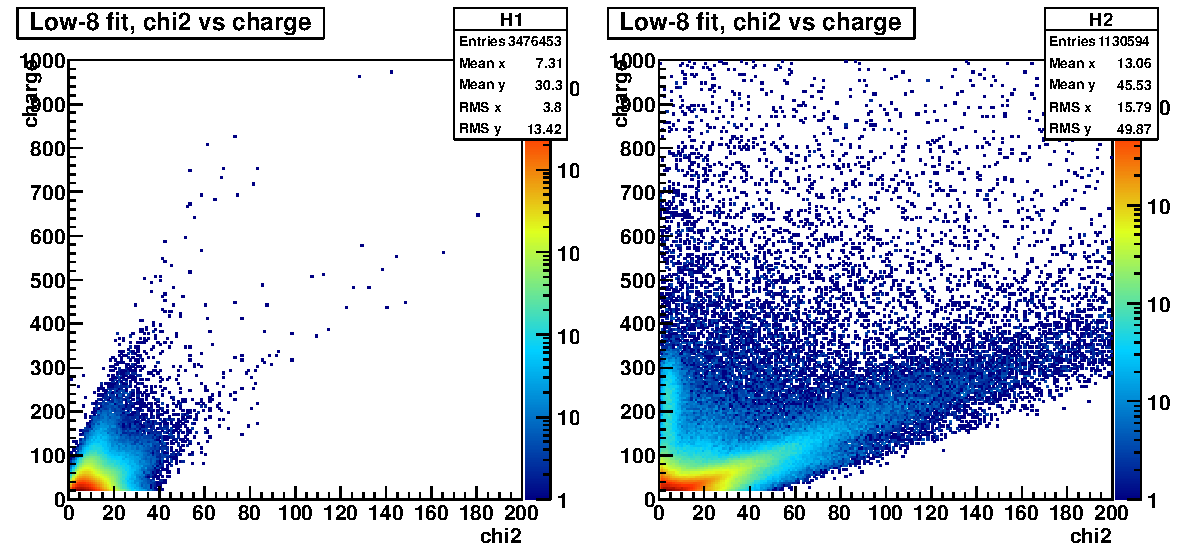
\includegraphics[width=120mm]{DailyLog/6324/6324HLow8FitChi2VsCharge.pdf}
   \caption{Low-8 fit chi2 vs. charge}
   \label{Figure_6324HLow8FitChi2VsCharge}
\end{figure}

\begin{figure}
   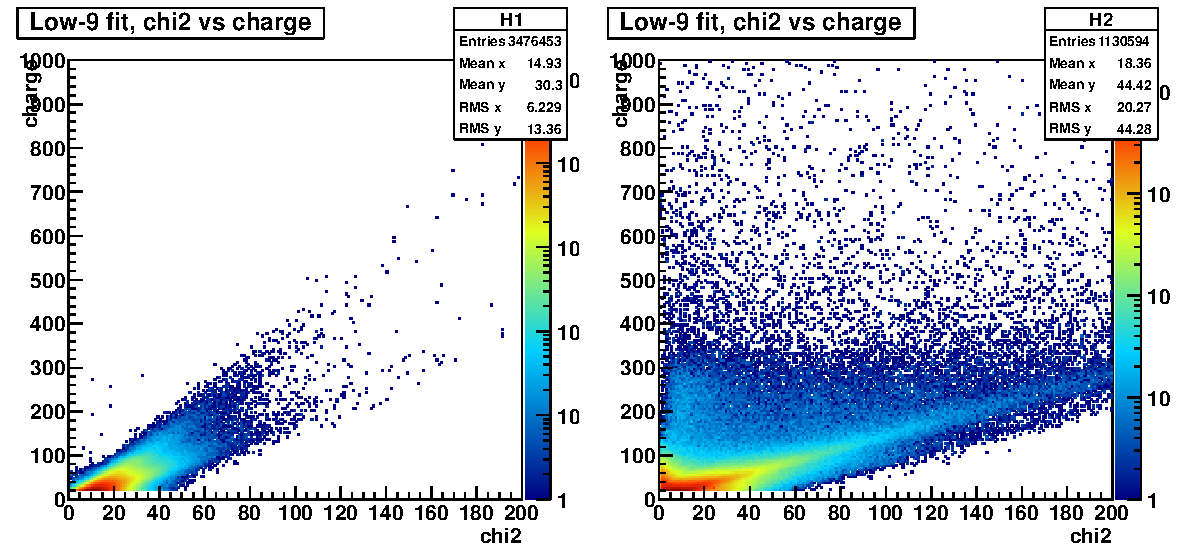
\includegraphics[width=120mm]{DailyLog/6324/6324HLow9FitChi2VsCharge.pdf}
   \caption{Low-9 fit chi2 vs. charge}
   \label{Figure_6324HLow9FitChi2VsCharge}
\end{figure}

\begin{figure}
   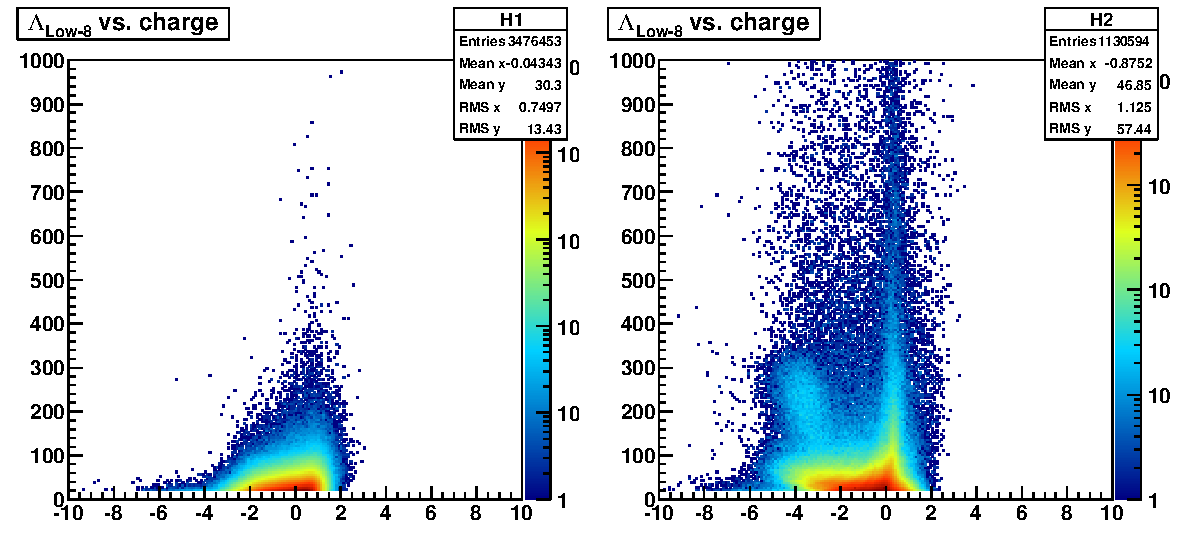
\includegraphics[width=120mm]{DailyLog/6324/6324HTestStatisticsLow8VsCharge.pdf}
   \caption{Low-8 fit test statistics vs. charge}
   \label{Figure_6324HTestStatisticsLow8VsCharge}
\end{figure}

\begin{figure}
   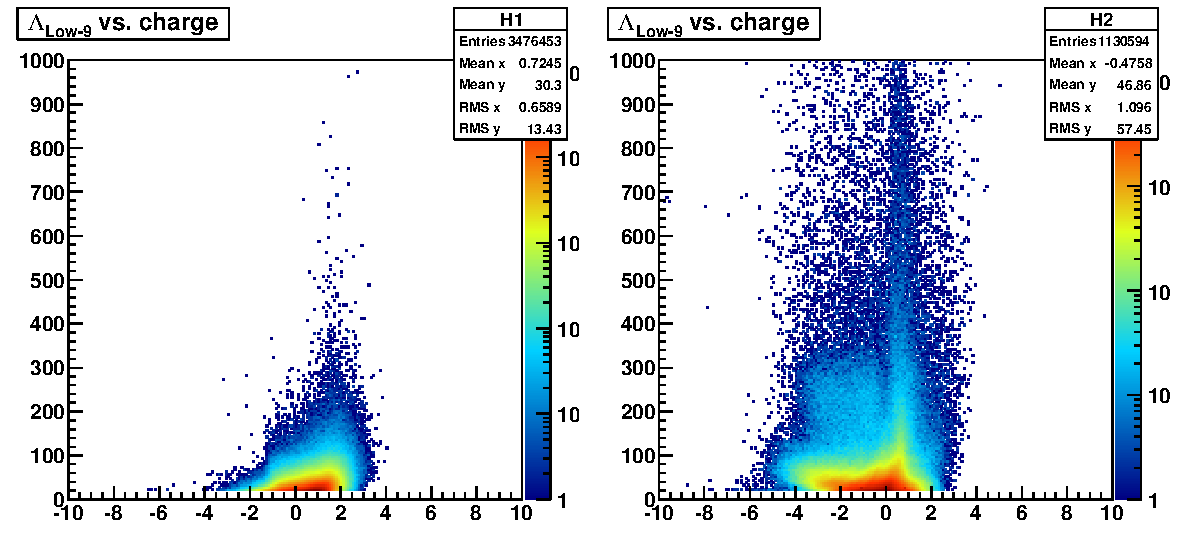
\includegraphics[width=120mm]{DailyLog/6324/6324HTestStatisticsLow9VsCharge.pdf}
   \caption{Low-9 fit test statistics vs. charge}
   \label{Figure_6324HTestStatisticsLow9VsCharge}
\end{figure}

\DailySection{Reflection}

\DailySection{Goals for next work day}

\begin{enumerate}
\item Eat lunch
\item Eat dinner
\item Find the red herring
\end{enumerate}


